\section{Fast Detector Simulation}\label{sec:ml4sim}

\subsection{Diffusion Models}\label{subsec:diffu}

Diffusion models are a type of generative AI, inspired by the physical process of diffusion.
Starting from some input data, such as images or calorimeter showers,
a training dataset is built by deterministically adding different amounts of noise to each image.
(Here, the term ``noise'' refers to (pseudo)random values that follow a Gaussian distribution;
it is not related to detector or electronics noise.)
Because the amount of noise in each training image is known, the diffusion model can learn how to add noise to the data.
The objective of the model is simply a regression task, and therefore the training converges reliably.
Figure~\ref{fig:illus} shows how adding noise repeatedly, over many iterations, produces an image that is pure noise.
To generate new images, this process is reversed, starting from pure noise to produce realistic data (``denoising'').

\begin{figure}[htb!]
\centering
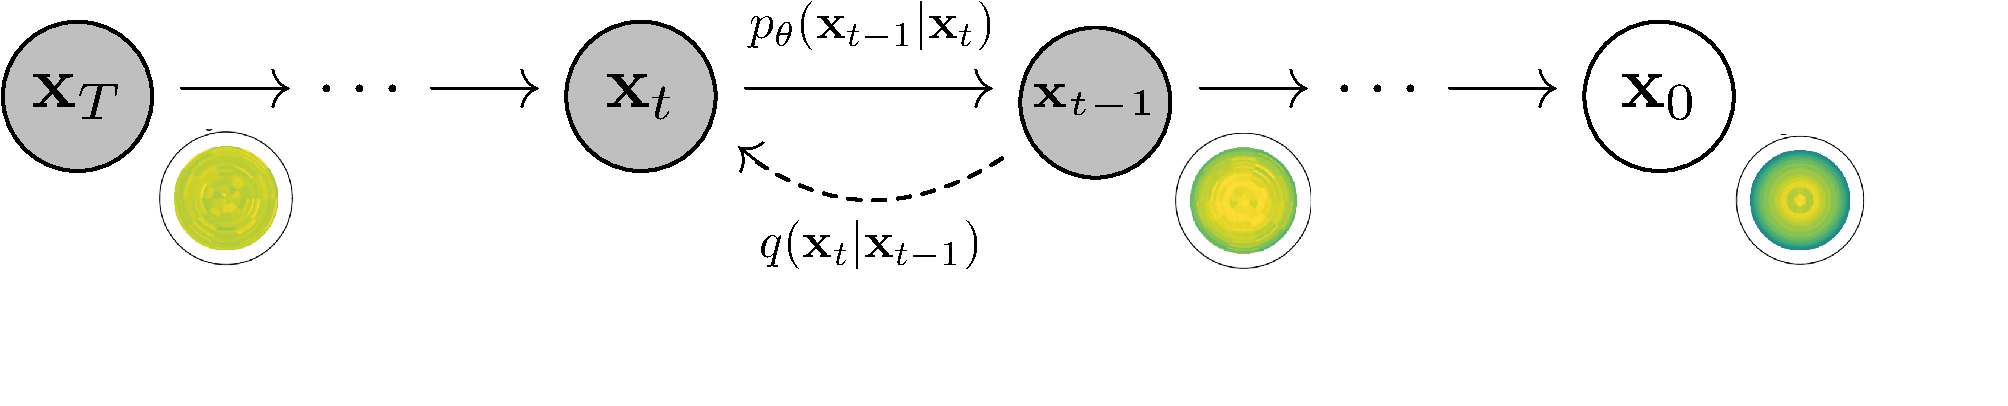
\includegraphics[width=0.95\myfigurewidth]{figures/pgm_diagram_xarrow_showers.pdf}
\caption{An illustration of the diffusion process, going from pure noise (left) to a realistic particle shower (right) in a transverse slice of a calorimeter. Adapted from Ref.~\cite{Ho:2020}.}
\label{fig:illus}
\end{figure}

The PI and his team developed the \diffu algorithm for the \challenge,
a recent community effort to compare different AI approaches to the simulation of particle showers in calorimeters, using common datasets and metrics.
The datasets include sampling calorimeters with varying materials and granularities and different particles including photons, pions, and electrons.
\diffu uses a convolutional U-net architecture~\cite{Ronneberger:2015}, along with several innovations to handle the non-rectangular and sometimes irregular geometry of calorimeters.
The convolution operations are \textit{cylindrical}, accounting for periodicity in the azimuthal angle $\phi$.
The convolutions are \textit{conditional} on the longitudinal and radial coordinates, to account for violations of translation invariance in particle shower evolution.
Finally, a novel approach called Geometry Latent Mapping (\glam) is employed:
the model can learn two matrices that map between the calorimeter's irregular geometry and a regular grid suitable for convolutions.
Figure~\ref{fig:calodiffu} (left) shows results from the \challenge on the pion dataset, clearly demonstrating the superiority of \diffu,
which is found to produce the highest quality showers for all datasets~\cite{Krause:2023mlj}.
The algorithms are compared based on metrics including classifier scores and the Fr\'echet particle distance~\cite{Kansal:2022spb}.
This version of the algorithm is published in Ref.~\cite{Amram:2023onf};
subsequently, the quality has been improved even further, as shown in Fig.~\ref{fig:calodiffu} (right), by adding a separate module that learns the per-layer deposited energy.

\begin{figure}[htb!]
\centering
\twofigeqh{figures/ds1-pions_CE_1.pdf}{figures/FCC_ERatio_dataset2_oct11_layer_norm_Diffu.pdf}
\caption{Left: example comparison of the separation power (for the shower center of energy) between \diffu, other algorithms, and \GEANTfour in the community \challenge.
Right: improved \diffu performance on the total deposited energy.}
\label{fig:calodiffu}
\end{figure}

The major remaining area for improvement in \diffu is its speed.
While it can still run 10--100 times faster than \GEANTfour by processing particles in large batches on GPUs,
the initial version required 400 denoising iterations or ``steps'' to produce high-quality output.
The improved version requires a factor of 4--8 fewer steps, depending on the dataset, because of its intrinsically higher quality.
More recently, some of the PI's colleagues have used \diffu as a platform to test further improvements to both the training and inference~\cite{Jiang:2024ohg},
and the most promising of these have been integrated into the model~\cite{Amram:GitHub}.
Numerous other avenues to make the algorithm faster while preserving quality are under investigation,
including latent diffusion~\cite{Rombach:2022}, consistency models~\cite{Song:2023}, and conditional distillation~\cite{Mei:2023}.
These illustrate a critical advantage of diffusion models:
because of the massive interest in these models in the broader ML community and in industry,
new methods are constantly being developed that can be easily imported for HEP use cases,
relying on the collaborative nature of open-source software.

Here, we propose to adapt \diffu to the more complex and variable CMS geometry.
The most involved case will be the High Granularity Calorimeter (HGCal), a part of the HL-LHC detector upgrades
that will increase the number of channels by almost two orders of magnitude.
The HGCal will have both hexagonal and rectangular cells in different regions, with different material types and thicknesses.
It is also the major driver of the predicted increase in \GEANTfour simulation time~\cite{Pedro:2020kbk}.
Further optimizations of the \diffu model will be needed to handle the high dimensionality and precision requirements of this new detector.
First, we will adapt the model to the existing, simpler CMS calorimeters,
which is both a useful stepping stone and an important ingredient for the dark QCD scan (Section~\ref{subsec:darkscan}).

\subsection{Refinement}\label{subsec:refine}

\begin{wrapfigure}[21]{L}{0.5\textwidth}
\centering
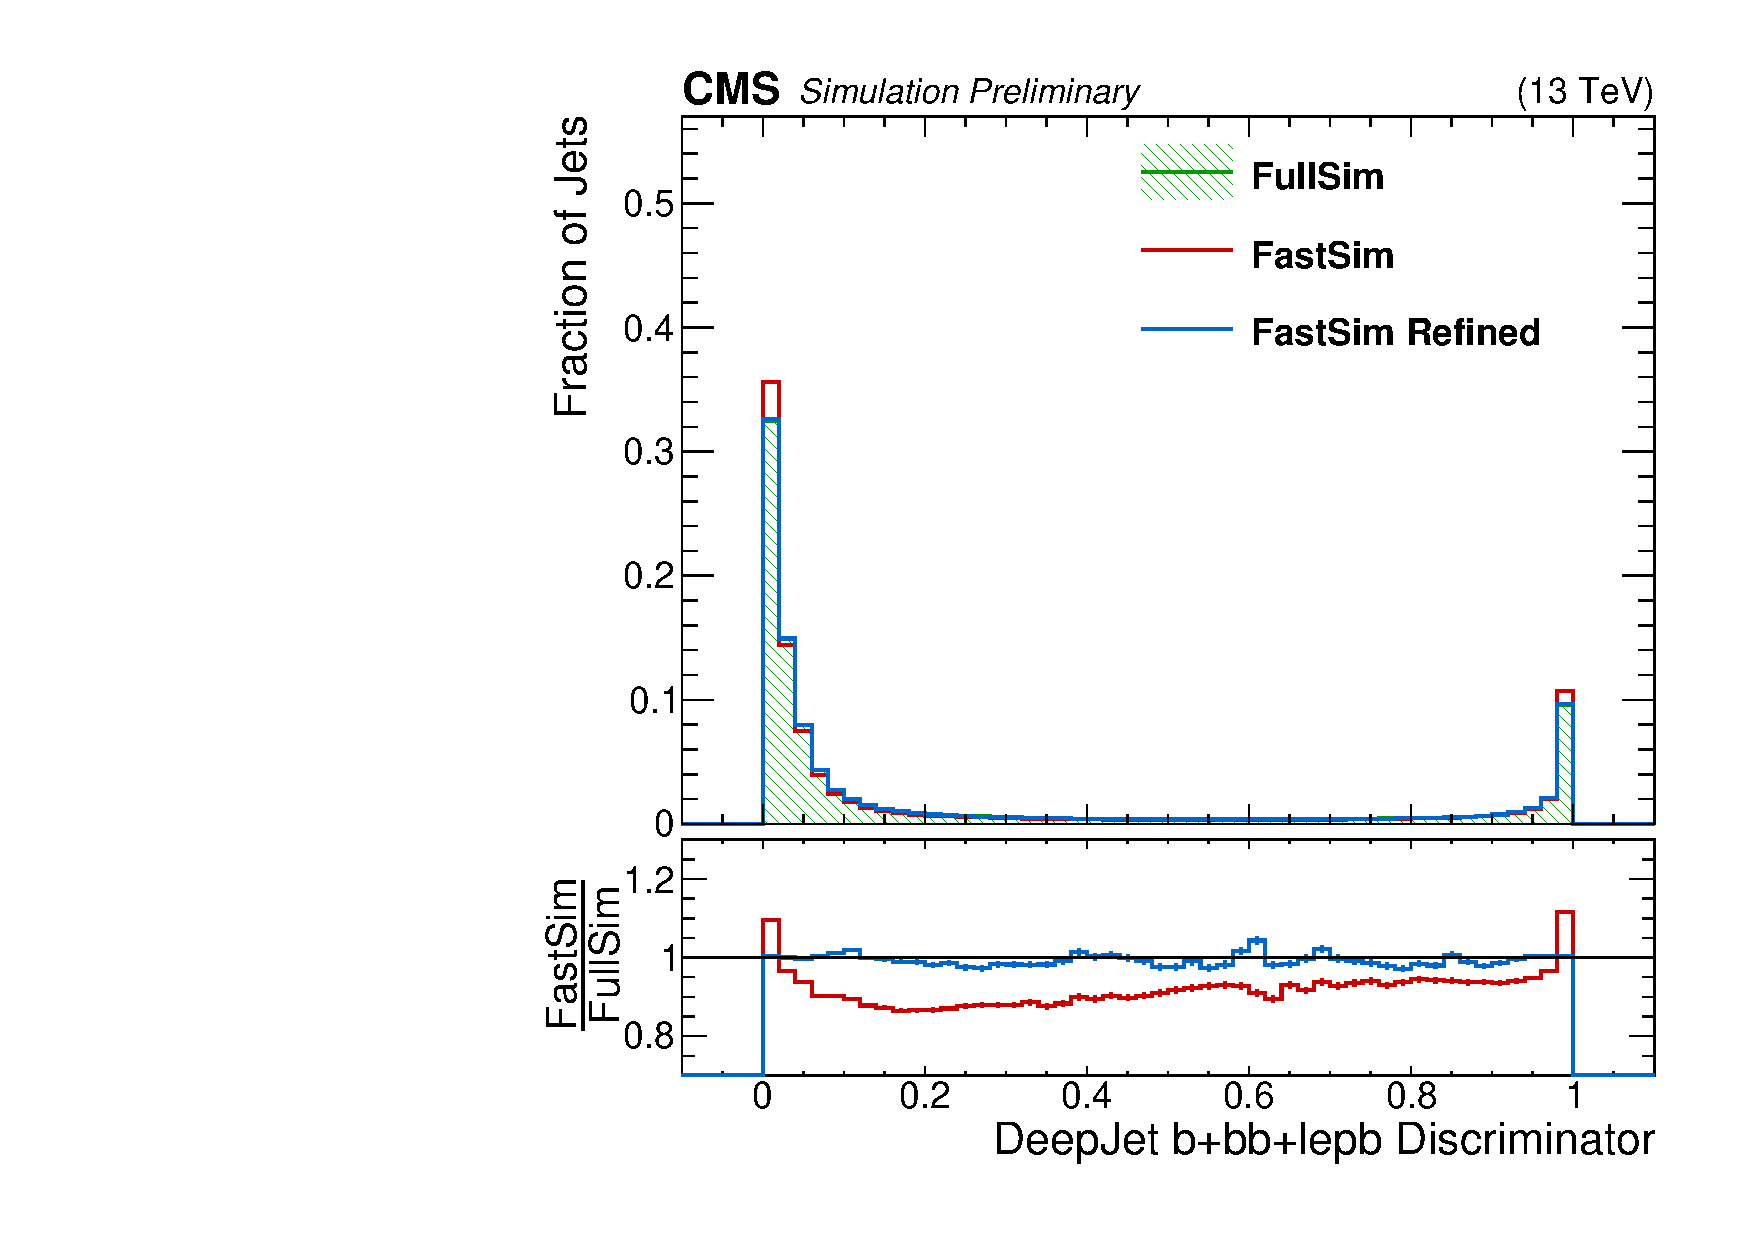
\includegraphics[width=0.49\myfigurewidth]{figures/Regression_20221127_DeepFlavB_preliminary.pdf}
\caption{The distribution of the \DEEPJET \cPqb-jet tagging discriminator, comparing \GEANTfour (FullSim), FastSim, and refined FastSim.}
\label{fig:refine}
\end{wrapfigure}

Conditional distillation is particularly interesting because it offers one path to enhance the existing CMS fast simulation chain (FastSim)~\cite{Sekmen:2016iql}.
Refining a low-quality simulation to obtain high-quality output was the objective of the PI's previous denoising project, which used a less sophisticated AI architecture~\cite{Banerjee:2022gkg}.
Diffusion models are much more capable, but so far the ``fully generative'' approach (producing a shower from pure noise) has been pursued;
this is because the sampling algorithms applied during the inference steps rely on the Gaussian nature of the noise.
The differences between FastSim and \GEANTfour will not be Gaussian, so while it is easier in principle to learn the difference between two similar distributions,
additional mathematical formalism must be derived in order to reuse the existing diffusion approach.
Instead, conditional distillation combines uses information from FastSim to supplement the fully generative approach, modifying the model to generate high-quality output in just one inference step.

The PI and his team have also developed a complementary high-level refinement, directly targeting analysis-level variables~\cite{Bein:2023ylt}.
This algorithm includes the first use of the modified differential method of multipliers~\cite{Platt:1987} in HEP,
which automatically balances a tradeoff between ensemble and per-event comparisons when training the network.
With promising results on \cPqb-jet tagging variables, shown in Fig.~\ref{fig:refine},
the algorithm is now being expanded to cover other jet-related variables and validated for use in Run 3.
The approach can be understood as a significantly more precise, correlation-preserving alternative to traditional, manually-calculated correction factors.
Given that the CMS FastSim currently only agrees with \GEANTfour to within ${\sim}10\%$,
high-level refinement alone can substantially reduce the quality deficits in FastSim samples and the resulting uncertainties.

The combination of diffusion and refinement will be even more powerful.
In the chain FastSim~$\to$~diffusion~$\to$~refinement, each ML algorithm solves a progressively easier problem,
because the difference with respect to the previous step is smaller.
Therefore, it can learn the solution more precisely from a given dataset size,
as well as incorporating physics at different levels (individual detector hits and reconstructed kinematic variables).
Essentially, refinement will address any residual disagreements between FastSim-based \diffu and \GEANTfour,
resulting in a more accurate final product, much like next-to-leading order matrix element calculations increase in accuracy by incorporating higher-order effects.

\subsection{Inference as a Service}\label{subsec:iaas}

As noted in Section~\ref{subsec:diffu}, the maximum speedup for AI-based simulation is achieved by performing inference on GPU
and generating showers for ${\sim}100$ particles simultaneously.
In order to reliably fill the GPU register, particles from multiple events must be processed together.
In addition, most CPUs in the Worldwide LHC Computing Grid currently are not directly connected to GPUs.
These considerations necessitate a flexible implementation of AI-based simulation algorithms in the experiment software framework.
As one of the only people to have implemented an alternative simulation engine in CMSSW~\cite{Pedro:2020kbk}
and the lead developer of the SONIC approach for inference as a service,
the PI has nearly unparalleled expertise in this area.

\begin{wrapfigure}[17]{r}{0.5\textwidth}
\centering
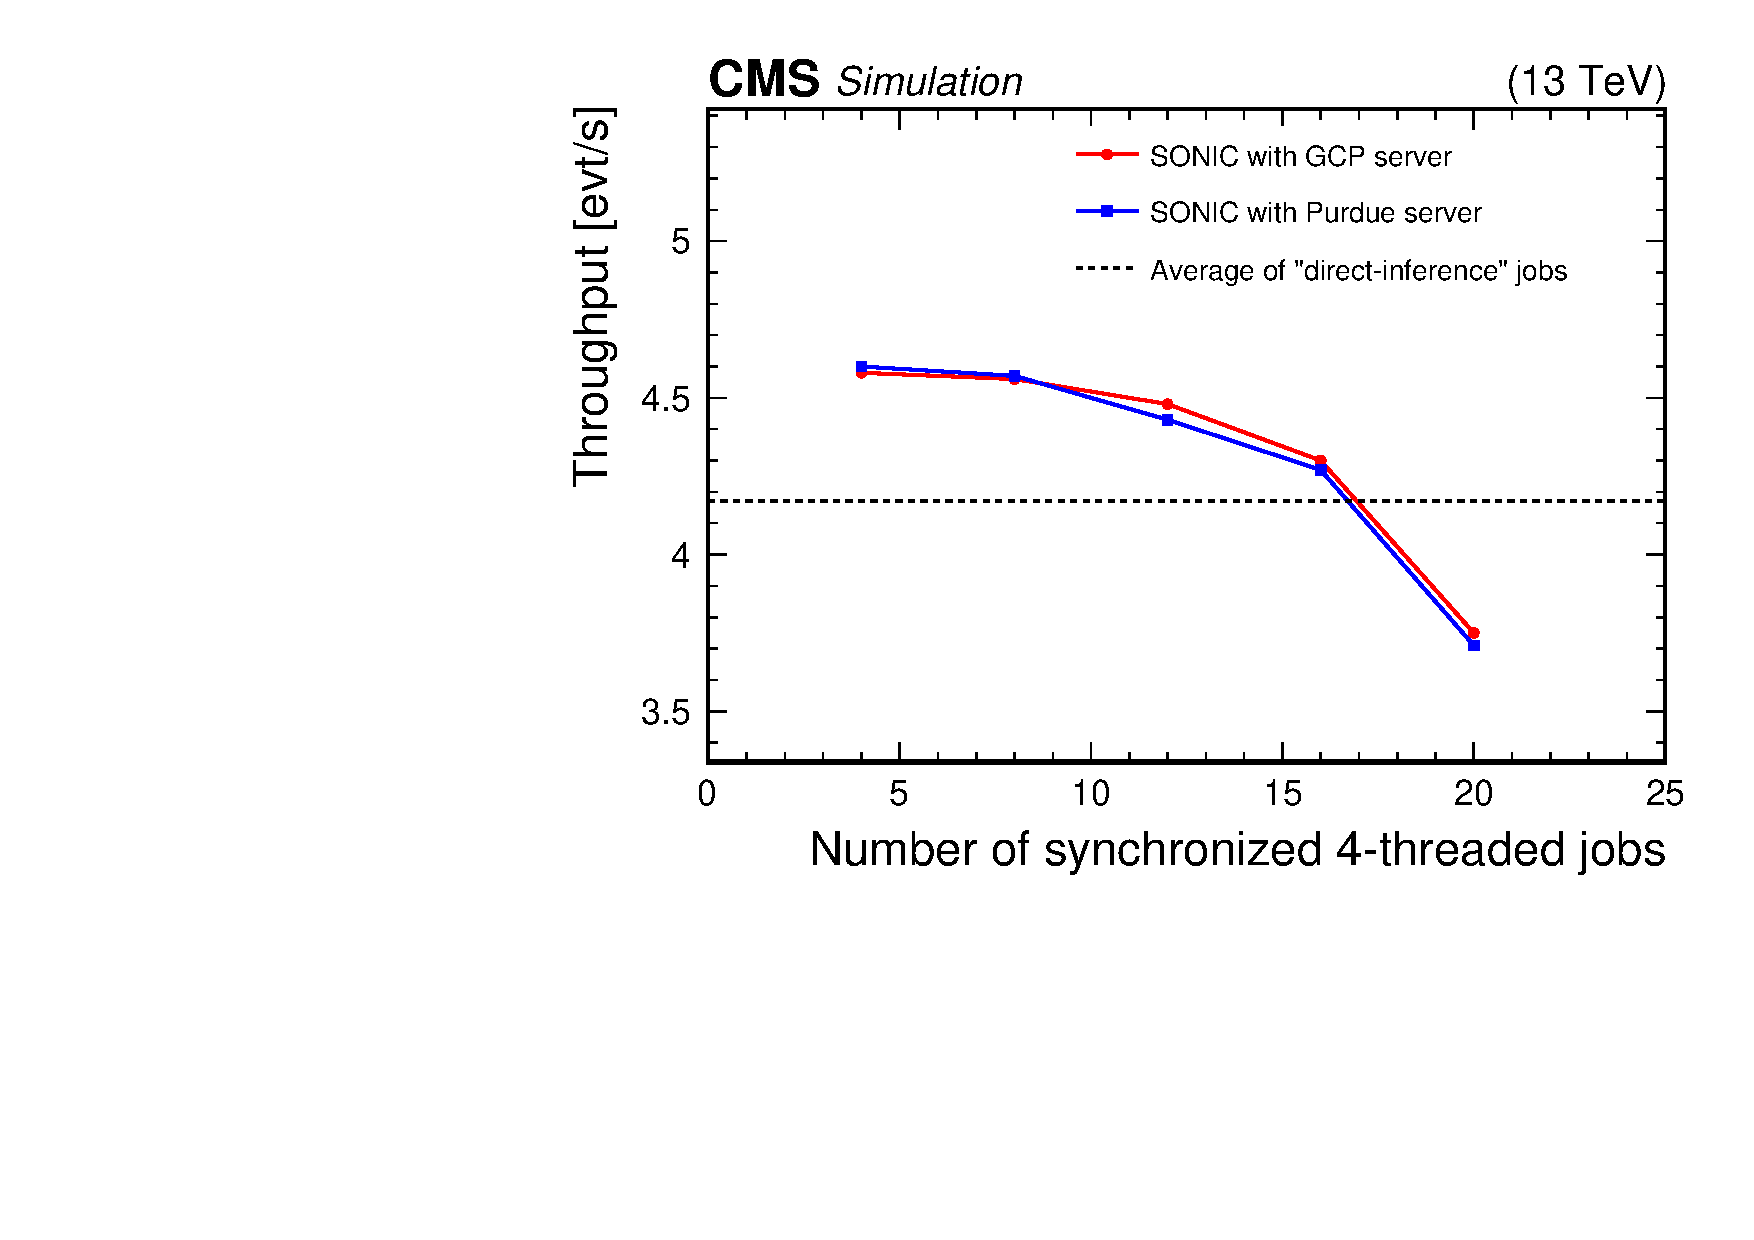
\includegraphics[width=0.49\myfigurewidth]{figures/MLG-23-001_Figure_009.pdf}
\caption{The event processing throughput for CPU-based workflows: without GPUs, with local GPUs, and with remote GPUs.}
\label{fig:sonic}
\end{wrapfigure}

SONIC enables access to heterogeneous coprocessor resources via a client-server approach
and has demonstrated inference acceleration by multiple orders of magnitude on GPUs, FPGAs, and intelligence processing units (IPUs).
Figure~\ref{fig:sonic} shows the most recent results for SONIC in CMS~\cite{CMS:2024twn}:
in an official data processing workflow, the use of GPUs completely eliminates the impact of AI algorithm inference on total throughput,
and the use of asynchronous, non-blocking requests~\cite{Bocci:2020olh} further eliminates the impact of client-server latency at least up to a distance of hundreds of kilometers.
SONIC minimizes programming and maintenance burdens while maximizing portability, efficiency, and accessibility.
A single coprocessor, located anywhere, can serve tens or even hundreds of CPU processes.
The underlying framework takes advantage of open-source tools, including the Nvidia Triton inference server~\cite{nvidia} and advances in machine learning packages.

The final product of this work is an AI-augmented simulation engine
that carries out rule-based algorithms on local CPUs and AI inference on remote GPUs via SONIC.
The fully generative diffusion model will be implemented within the \GEANTfour interface, in order to validate its performance against the highest quality simulation.
(A complete validation requires comparison of reconstruction-level quantities that can only be computed using the entire CMSSW processing chain.)
The FastSim-based diffusion model will be implemented within the CMS FastSim application, in combination with high-level refinement, to deliver the fastest high-quality simulation.
The technologies and innovations in this part of the proposal have mostly been proven to work in other contexts, as shown above.
Viable alternatives exist to mitigate the risks from the new elements:
\begin{enumerate}
\item \textit{Faster diffusion}: if the various approaches to speed up the fully generative diffusion model do not succeed, this will reduce the amount of simulation that can be produced, though it is still expected to exceed \GEANTfour when running in batches on GPU. As a fallback, the existing FastSim can be used in combination with high-level refinement to achieve some reduction in uncertainty.
\item \textit{FastSim-based diffusion}: if the combination of the diffusion model with the existing FastSim is not viable, the fully generative diffusion model can be used, or high-level refinement can be used alone (see above).
\item \textit{SONIC implementation}: if unforeseen complications are encountered in the use of inference as a service, directly-connected GPUs can be employed, at the cost of limiting the computing sites where simulation can be run effectively.
\end{enumerate}
The AI-augmented simulation engine will be ready by the end of Run 3 to enable the comprehensive dark QCD scan (Section~\ref{subsec:darkscan})
and to be employed for HL-LHC simulations for Run 4 and beyond.

\subsection{Future Colliders}\label{subsec:mucoll}

If a hidden valley exists but only couples to the SM via mediators at the 10\TeV scale, collider DM production will require a future, higher energy accelerator.
The new P5 report~\cite{P5:2023} specifically highlights a muon collider as an attractive option to reach parton center-of-mass energies of 10\TeV,
both because of its compact footprint and because of the numerous technological innovations and synergies that would be achieved in the course of constructing and operating this machine.
While the collider itself is several decades away, the report highlights that research and development must start now.
Simulation is a crucial component of the design process for both the detectors and the collider,
and the machine-detector interface (MDI) is particularly important for the muon collider.
The MDI must incorporate mitigations for the beam-induced background (BIB) caused by muon decays in flight as the beam circulates.
At $\sqrt{s_{\Pgm\Pgm}} = 10\TeV$, there are ${\sim}10^5$ muon decays per meter, leading to ${\sim}10^8$ photons and neutrons per bunch crossing~\cite{Black:2022cth}.

Currently, it takes 24 hours to simulate just one BIB event with \GEANTfour.
AI-based BIB simulation, therefore, would be highly impactful for muon collider, detector, and MDI design.
While \diffu is trained on single-particle events, because material interactions in \GEANTfour are modeled independently for every particle,
it may not be feasible to continue such an approach for events with $10^8$ particles.
This can be addressed by implementing a ``grouped'' approach, in which similar particles are grouped together to train the diffusion model to generate their energy deposits together.
However, as previously noted, the output of the diffusion model must be validated by comparison to full simulation to ensure its reliability.
It is a challenging prospect for \GEANTfour even to produce a sufficient validation sample at these multiplicities.
This is an area where the new GPU-based simulation engine Celeritas offers several advantages.
The physics processes by which photons and neutrons deposit energy are limited,
with electromagnetic (EM) processes already implemented in Celeritas and neutron transport implemented in its predecessor Shift~\cite{Hamilton:2018}.
The staggering multiplicity of BIB particles will ensure efficient use of GPUs for optimal throughput.
In these conditions, Celeritas may provide up to a factor 40 speedup compared to \GEANTfour~\cite{Tognini:2022nmd}.

After further refinement of \diffu using CMS calorimeter datasets of widely varying complexity,
we will apply the algorithm to simulate BIB for muon collider detector design.
The results will be validated against Celeritas simulations incorporating EM and neutron physics and the MDI geometry.
Based on existing results, we expect \diffu to provide a significant speedup even compared to Celeritas.
This combination of new approaches to simulation illustrates another facet of the synergies in the proposed muon collider program.
Further, given that BIB events also consume substantial disk space, 8--36 GB per event,
encoding this information in a diffusion model can be considered a form of compression:
the model trades disk usage for computing power by being able to generate BIB events on the fly,
requiring only $\mathcal{O}(\text{MB})$ learned weights and a source of randomness.
This novel application of AI-based simulation will facilitate improved designs and
better projections of the physics potential of the next generation of the energy frontier.